%%%%%%%%%%%%%%%%%%%%%%%%%%%%%%%%%%%%%%%%%%%
%%% DOCUMENT PREAMBLE %%%
%This template was adapted from a template by Roza Aceska.
\documentclass[12pt]{report}
\usepackage[english]{babel}
%\usepackage{natbib}
\usepackage{url}
\usepackage[utf8x]{inputenc}
\usepackage{amsmath}
\usepackage{graphicx}
\usepackage{parskip}
\usepackage{fancyhdr}
\usepackage{vmargin}
\usepackage{caption}
\usepackage{subcaption}

\usepackage{tabularx}
\usepackage{xcolor,colortbl}
\newcommand{\notimportant}{\cellcolor{black!10}x} 
\usepackage{hyperref}
\usepackage{cleveref}
\usepackage{float}

\setmarginsrb{3 cm}{2.5 cm}{3 cm}{2.5 cm}{1 cm}{1.5 cm}{1 cm}{1.5 cm}

\title{Report Assignment Part 2}
% Title
\author{}						
% Author
\date{17.07.2020}
% Date

\makeatletter
\let\thetitle\@title
\let\theauthor\@author
\let\thedate\@date
\makeatother

\pagestyle{fancy}
\fancyhf{}
\rhead{\theauthor}
\lhead{\thetitle}
\cfoot{\thepage}
%%%%%%%%%%%%%%%%%%%%%%%%%%%%%%%%%%%%%%%%%%%%
\begin{document}

%%%%%%%%%%%%%%%%%%%%%%%%%%%%%%%%%%%%%%%%%%%%%%%%%%%%%%%%%%%%%%%%%%%%%%%%%%%%%%%%%%%%%%%%%

\begin{titlepage}
	\centering
    \vspace*{0.5 cm}
  \begin{center}    \textsc{\Large   Adavanced Process Mining SS20}\\[2.0 cm]	\end{center}
	\rule{\linewidth}{0.2 mm} \\[0.4 cm]
	{ \huge \bfseries \thetitle}\\
	\rule{\linewidth}{0.2 mm} \\[1.5 cm]
	
  \begin{minipage}{0.48\textwidth}
    \begin{flushleft} \large
      \emph{Submitted To:}\\
      Tobias Brockhoff\\
      Lisa Mannel\\
      Sebastiaan J. van Zelst MSc PhD\\
    \end{flushleft}
  \end{minipage}~
  \begin{minipage}{0.48\textwidth}
    \begin{flushright} \large
			\emph{Submitted By:} \\
      Sezin Maden (354463) \\
      Bruno Machado Pacheco (403532)  \\
      Tom-Hendrik Hülsmann (355773)
		\end{flushright}
	\end{minipage}\\[2 cm]
	
\end{titlepage}

%%%%%%%%%%%%%%%%%%%%%%%%%%%%%%%%%%%%%%%%%%%%%%%%%%%%%%%%%%%%%%%%%%%%%%%%%%%%%%%%%%%%%%%%%

\renewcommand{\thesection}{\arabic{section}}

\section{Q1. Preliminary Analysis}

\paragraph{\textbf{a)}}
We begin our analysis by creating two sub-logs of the original event log. One sub-log that contains all cases that did have an appeal and one sub-log containing all cases that did not have an appeal. The distinction between such cases is made based on events that are related to appeals. We know that there are two ways in which an offender can appeal. There either is an appeal to the prefecture or to a judge. The two relevant events that indicate an appeal on the side of the police department are \texttt{Appeal to Judge} and \texttt{Send Appeal to Prefecture}. The two sub-logs are created by filtering the original log based on these events using pm4py. Traces that contain either of these events are either discarded or kept depending on the sub-log.

\paragraph{\textbf{b)}}
For the three logs obtained in the previous step, we compute some core descriptive metrics. All of the resulting values can be found in \ref{tab:1b}.
\begin{table}[H]
\centering
\begin{tabular}{|l|l|l|l|l|}
	\hline \textbf{Metric} & \textbf{Complete} & \textbf{Only Appeals} & \textbf{Without Appeals} \\
	\hline Number of Traces & 150,370 & 4,513 & 145,857\\
	\hline Number of Variants & 231 & 170 &61\\
	\hline Number of Events & 561,470 & 29,724 & 531,746\\
	\hline Average Trace Length & 3.73 & 6.59 & 3.65\\
	\hline First Event Date & 01.01.2000 & 03.01.2000 & 01.01.2000\\
	\hline Last Event Date & 18.06.2013 & 14.06.2013 & 18.06.2013\\
	\hline Number of Activities & 11 & 11 & 9 \\
	\hline Traces with Duplicate Activities  & 0.0812 \% & 0.0252 \% & 0.0843 \%\\
	\hline
\end{tabular}
\caption{Some basic Metrics of the three event logs.}
\label{tab:1b}
\end{table}
The \emph{Number of Traces}, \emph{Number of Events} and \emph{Number of Activities} metrics were obtained through the \emph{Log Summary} feature of ProM. The \emph{Number of Variants}, \emph{Average Trace Length} and \emph{First/Last Event Date} were computed using the \emph{Explore Event Log} feature of ProM. Additionally the number of traces that are containing duplicate activities were computed using a custom Python script.

\paragraph{\textbf{c)}}

An overview of the relative frequency of all activities in the three logs can be seen in figure \ref{fig:activity_frequencies}. The raw frequency values can be found in the appendix in table \ref{tab:1c_absolut} and table \ref{tab:1c_relative}. The values were obtained using the \emph{Log Summary} feature of ProM. 
\begin{figure}[H]
  \centering
  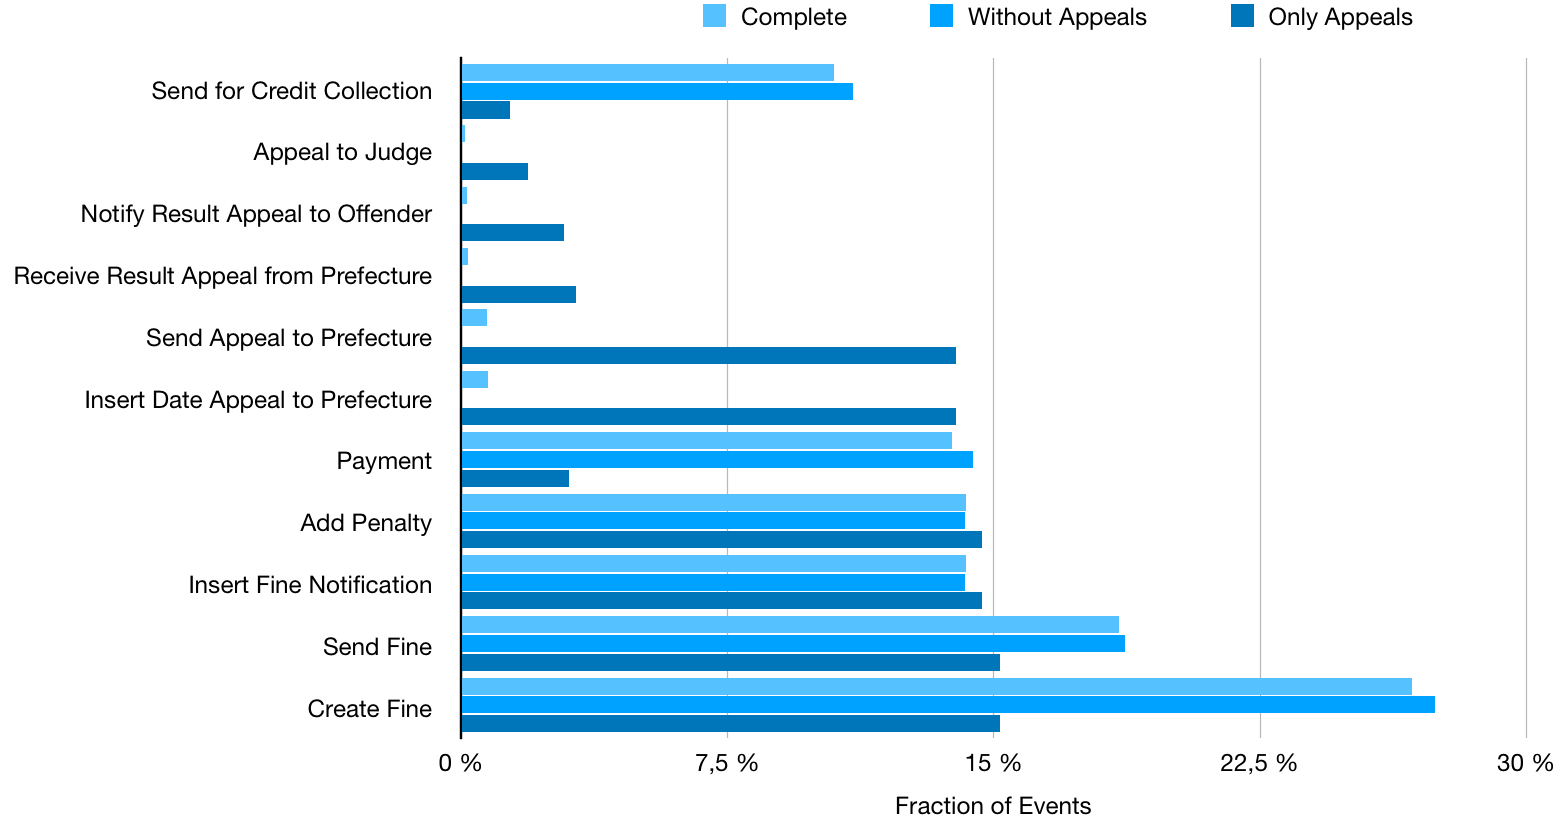
\includegraphics[width=\textwidth]{figures/activity_frequencies.png}
  \caption{The fraction of events of each log grouped by activity.}
  \label{fig:activity_frequencies}
\end{figure}

Also using the ProM \emph{Log Summary} feature, it was found that for all three event logs, 100\% of the traces start with the \texttt{Create Fine} activity. The relative frequencies of end activities can be found in figure \ref{fig:end_frequencies}. The exact values for the end activity frequencies can be found in the appendix in table \ref{tab:1c_end}. 
\begin{figure}[H]
  \centering
  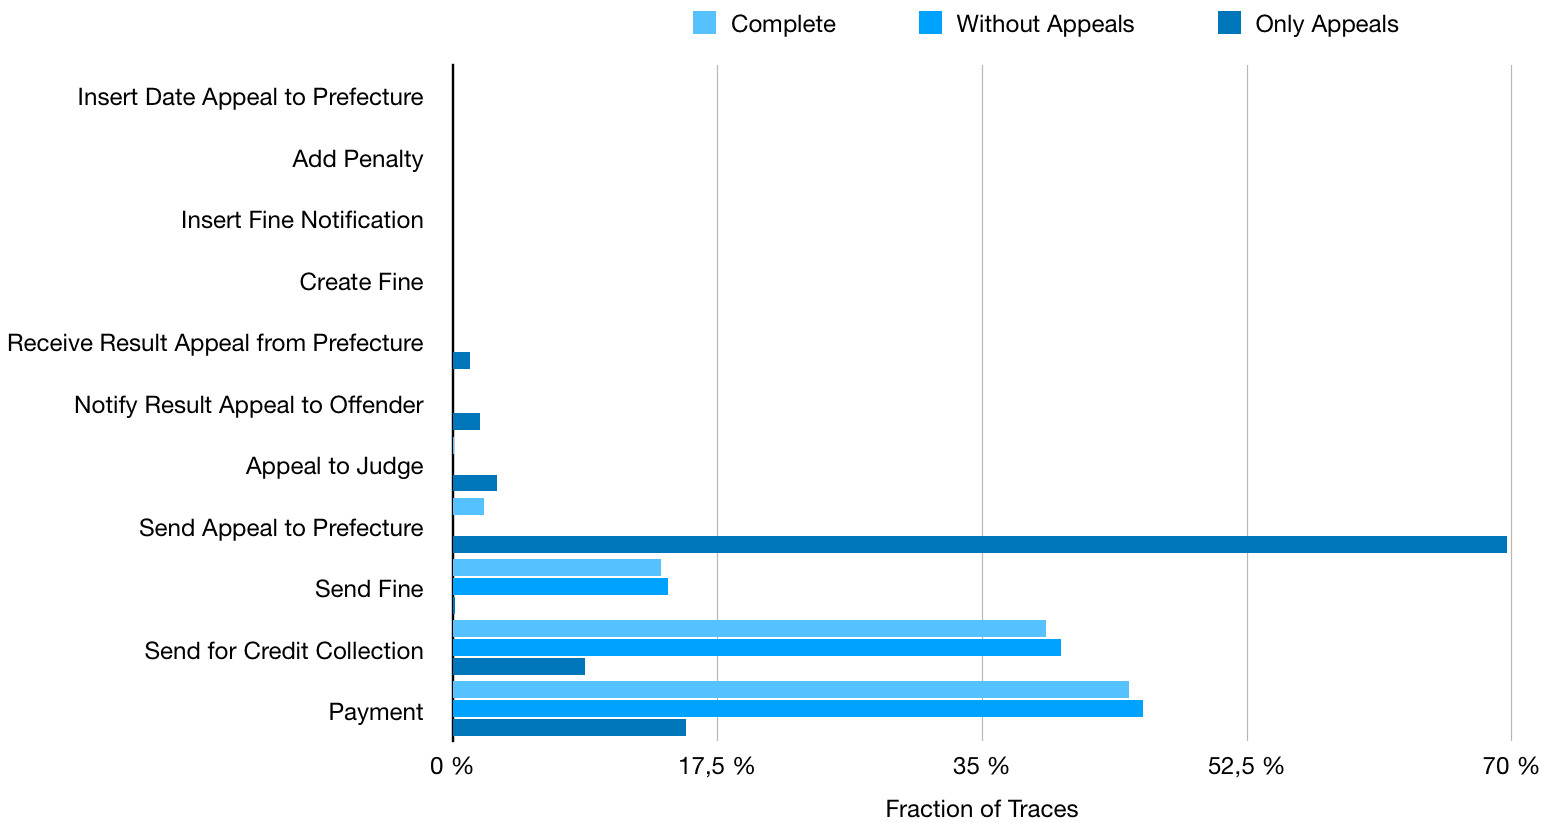
\includegraphics[width=\textwidth]{figures/end_frequencies.png}
  \caption{The fraction of Traces that end with the specified activity in each of the three event logs.}
  \label{fig:end_frequencies}
\end{figure}

\paragraph{\textbf{d)}} In order to to be able to see the different activity types over time, two dotted charts over the events were created. This was done by importing the filtered event log, containing only cases that did not have an appeal, into ProM. There, the \emph{LogProjection} plugin was used in order to create the two visualizations. The first chart that can be seen in figure \ref{fig:dotted_timestamp} shows the different activity types on the y-axis.
For each event, a dot is visible at the point in time when the event occurred. We can therefore observe which types of activities were performed at which time over the whole timespan of the log. In general we can see that there are two main types of activities. Those activities that are performed constantly throughout the year, and those that only occur infrequently. The continually performed activities consist of \texttt{Add Penalty}, \texttt{Create Fine}, \texttt{Insert Fine Notification}, \texttt{Payment} and \texttt{Send Fine} activities. Of those, the \texttt{Create Fine} and \texttt{Payment} activities have no gaps and are therefore always performed. The remaining continuous activities show some gaps over the years. These gaps do not seem to follow a particular pattern and are spread throughout the year. However we see, that the gaps of these activities coincide with each other somehow. The \texttt{Insert Date Appeal to Prefecture}, \texttt{Notify Result Appeal to Offender}, \texttt{Receive Result Appeal from Prefecture} and \texttt{Send for Credit Collection} activities occur much less frequent. The \texttt{Send for Credit Collection} activity seems to only occur once every year, mostly near the beginning or end of the year. The \texttt{Notify Result Appeal to Offender} and \texttt{Receive Result Appeal from Prefecture} activities only start appearing for the first time in 2007, in contrast to the other activities which occur from the beginning of the log. This suggest that they represent a new branch of the process that was introduced in 2007.
\begin{figure}[H]
  \centering
  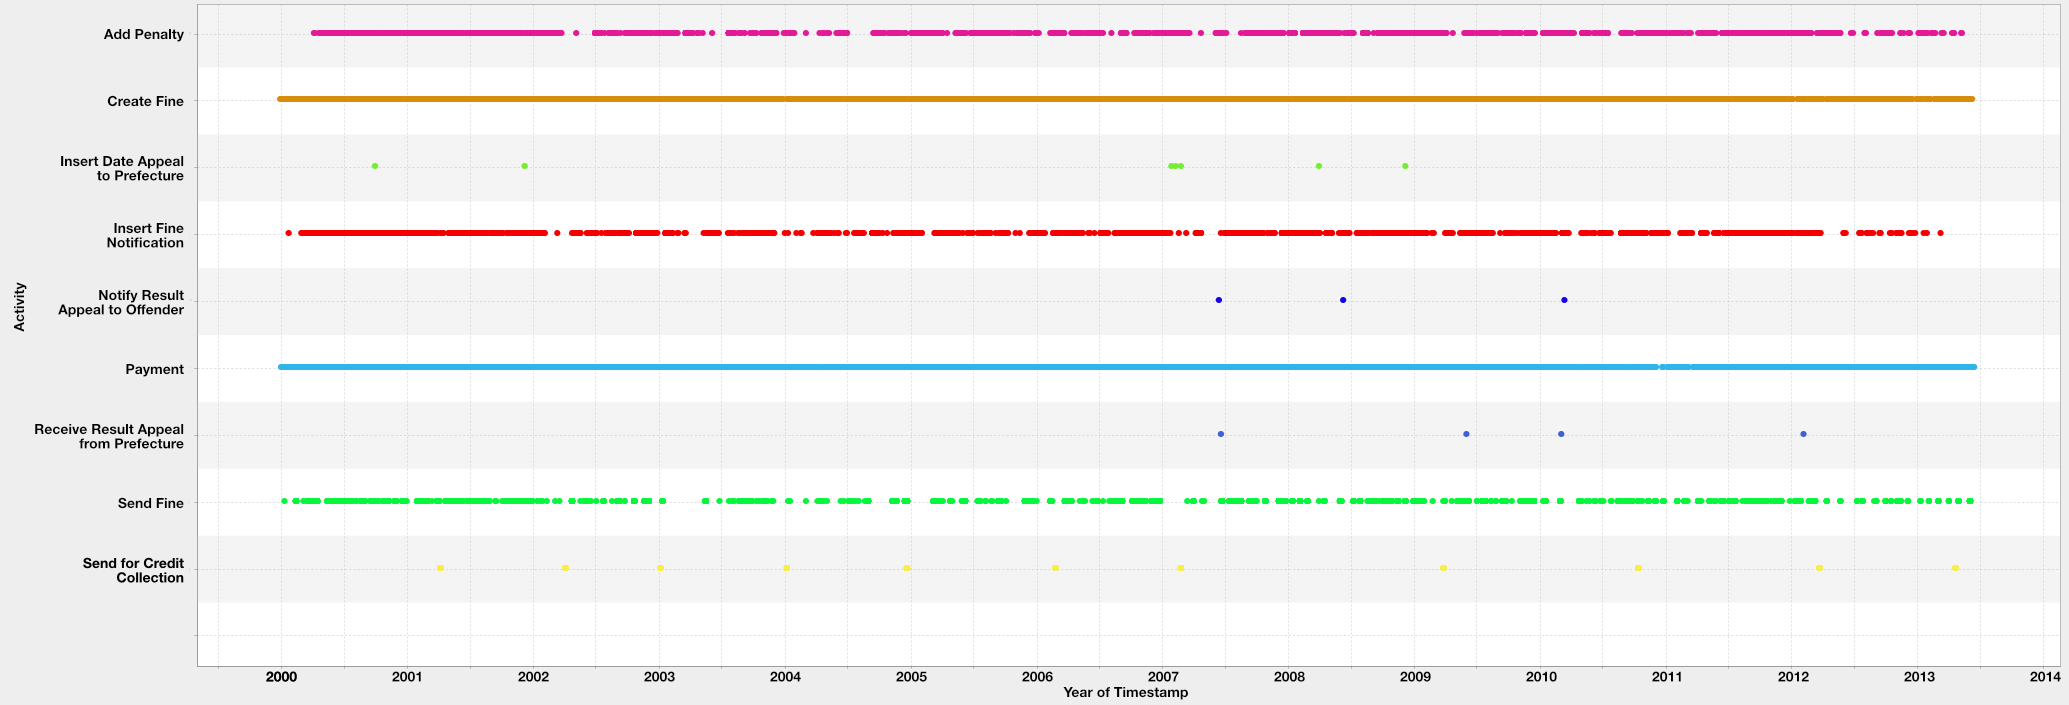
\includegraphics[width=\textwidth]{figures/dotted_timestamp.png}
  \caption{Event occurrences for cases without an appeal, grouped by activity type over time.}
  \label{fig:dotted_timestamp}
\end{figure}

The second chart that can be seen in figure \ref{fig:dotted_duration} also shows the different activity types on the y-axis. However the events are now plotted over the case duration at the time that the event occurred. This case duration metric was automatically computed by the used \emph{LogProjection} plugin. We see that \texttt{Create Fine} is always the first event of every case, as was already discovered in \textbf{c)}. The activity is therefore only observable at the beginning of the chart. \texttt{Send for Credit Collection} activity only starts after almost a full year of case duration and is the activity that is performed the latest in most cases. The first activity after one year can be explained with the findings from the previous chart, where it was discovered that the activity is only performed once a year. The \texttt{Payment} activity also has some events performed in late stages of the process instances, but is also frequent throughout all case durations. The other activities are mostly performed within the first year of an active case. The \texttt{Notify result Appeal to Offender} activity is always performed before the \texttt{Receive Result Appeal from Prefecture} activity. Overall we can see that the activities that are performed directly by the police department occur earlier in the cases or in cases that have an overall shorter duration. Activities that are depending on the offender and are related to payments appear at the very end of the case. The longest case durations are therefore caused by cases in which the offender makes a delayed payment. It is also visible that the frequent events are mostly spread across the whole range of case durations, with only a small reduction towards the extremely long case durations. This suggests that there are no peaks in case duration and there is an almost equal distribution of case durations over the timeframe.

\begin{figure}[H]
  \centering
  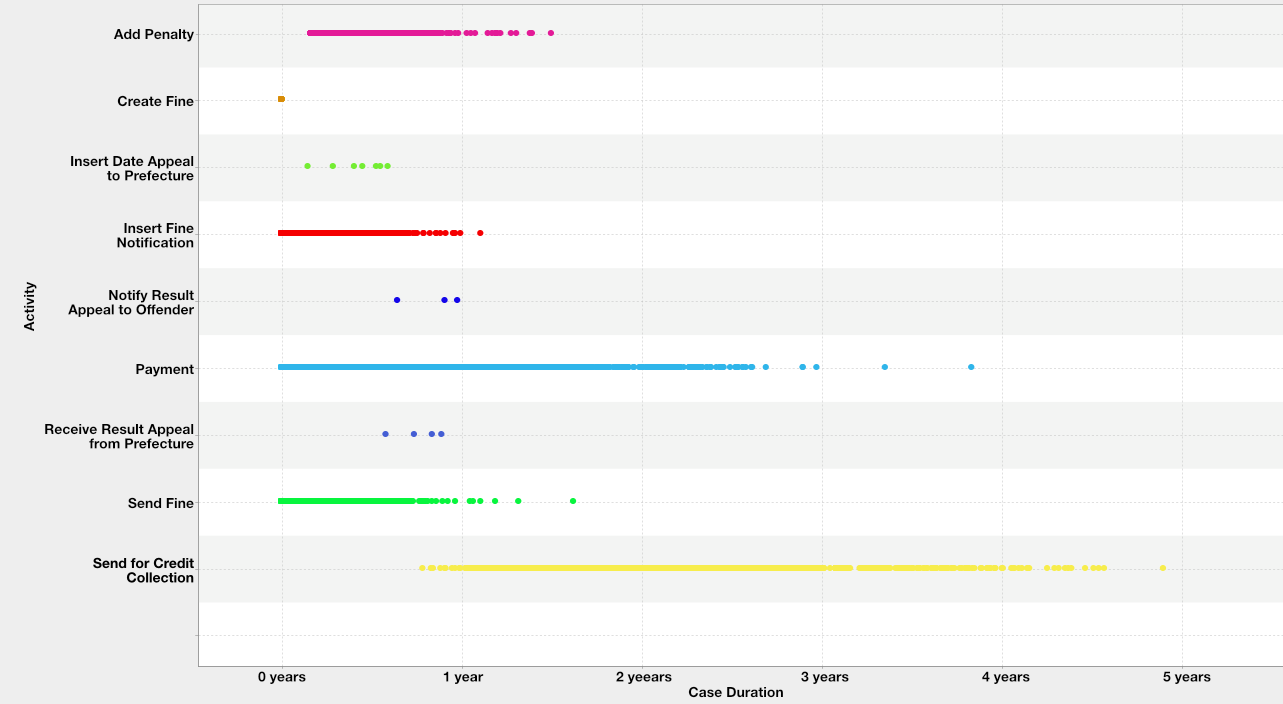
\includegraphics[width=\textwidth]{figures/dotted_duration.png}
  \caption{Event occurrences for cases without an appeal, grouped by activity type over the case duration at the time the event occurred.}
  \label{fig:dotted_duration}
\end{figure}

\paragraph{\textbf{e)}}

Based on table \ref{tab:1b} we can now compare the three logs according to some basic metrics. We see that the majority of
cases do not contain any appeal, with only around $3\%$ of the traces having an appeal. The average trace length of appeal cases is almost twice as long as for cases without appeal. Because of this, the cases are over represented regarding the number of events, with about $5\%$ of events in the original log being related to appeal cases. Using figure \ref{fig:activity_frequencies} we observe that most of these appeal cases are appeals to the prefecture. There are seven times as many appeals to the prefecture as there are appeals to a judge.  The variety of traces is much higher in the log containing only appeals. On average there are 100 times more traces for each variant in the log without appeals compared to the log with appeals. This means that a majority of trace variety in the log is explained by only a small number of traces with an appeal. This can be explained by the longer average trace length of these cases, which leads to more variant possibilities. Although the log with only appeals has a higher average trace length, it contains far less traces with duplicate activities than the other two logs, which is surprising. This can probably be explained by the fact that appeals processes involve additional events that are not possible for non appeals processes. We see that the original log has the same timeframe as the log without appeals. The log consisting of only appeals cases however starts two days later and ends four days prior. This can most likely be explained by the lower amount of cases that have an appeal, so that in the missing time, no events for such cases occurred. The number of activities is the same for the original log and the log containing only appeals cases. This means that there are no activities that are only performed for cases without appeals. As expected there are less activities in the log containing no appeals, as the events on which the filtering was based are no longer present.

In addition to the above findings, a closer look was given at the relative frequencies of specific activities in figure \ref{fig:activity_frequencies} and figure \ref{fig:end_frequencies}. As mentioned above we observe that the \texttt{Appeal to Judge} and \texttt{Send Appeal to Prefecture} activities are missing from the log without appeals because of the filtering. However there are still some activities left that are related to the appeals process and in theory should therefore only present in the log containing the appeals. These activities are \texttt{Insert Date Appeal to Prefecture}, \texttt{Receive Result Appeal from Prefecture} and \texttt{Notify Result Appeal to Offender}. A closer inspection of these traces reveals that in half of the instances, a payment was made directly after the \texttt{Insert Date Appeal to Prefecture} activity. This suggests that the offender was planning on appealing, but payed the fine before the appeal was send to the prefecture. These traces are therefore most probably correct and are correctly assigned to the sub-log as indeed there was no appeal.  However in the other half of cases, the appeals process was complete, with receiving a result from the prefecture and notifying the offender. In these cases only the \texttt{Send Appeal to Prefecture} activity is missing, which suggests that these are recording errors in the log, because it is not possible to receive an answer from the prefecture without sending the appeal first. So most probably it was missed to record the sending activity.

An open question that could point to a possible problem is the high amount of traces containing \texttt{Send for Credit Collection} in the log without appeals. Especially when keeping in mind that this activity is batched together. It is very likely that the average case duration could be reduced if there were less cases where the fine has to be collected externally. The same observation can also be made in figure \ref{fig:end_frequencies}. Furthermore, in the cases without appeals there are many traces ending with a \texttt{Send Fine} activity, which points to a high number of unpaid fines. Further analysis should investigate if this suspicion is true and what can be done to counter it. Regarding the end activities it is also interesting that of the appeal cases, almost $70\%$ end with the \texttt{Send Appeal to Prefecture} activity. This is unexpected, as this is not a wanted end activity. This leads to the assumption that these cases are not yet finished and are still waiting for the next event to occur. To check this, we look at the distribution of these traces over time. If these are cases that were not yet finished before the end of the considered timeframe, we would expect them to pool at the end of the timeframe. This is however not the case, the cases are spread evenly over the timeframe. Therefore the cases are most probably actually finished. Further investigation reveals that in most cases where the end activity was not \texttt{Send Appeal to Prefecture}, an actual payment was made or the case was sent for credit collection. This suggests that the case is only passed back to the police department in cases in which the appeal is discarded. This means that the appeals of the cases ending in \texttt{Send Appeal to Prefecture} were most probably successful appeals.

\section{Q2. Discovery and Conformance}

\paragraph{\textbf{a)}}
\begin{figure}[H]
  \centering
  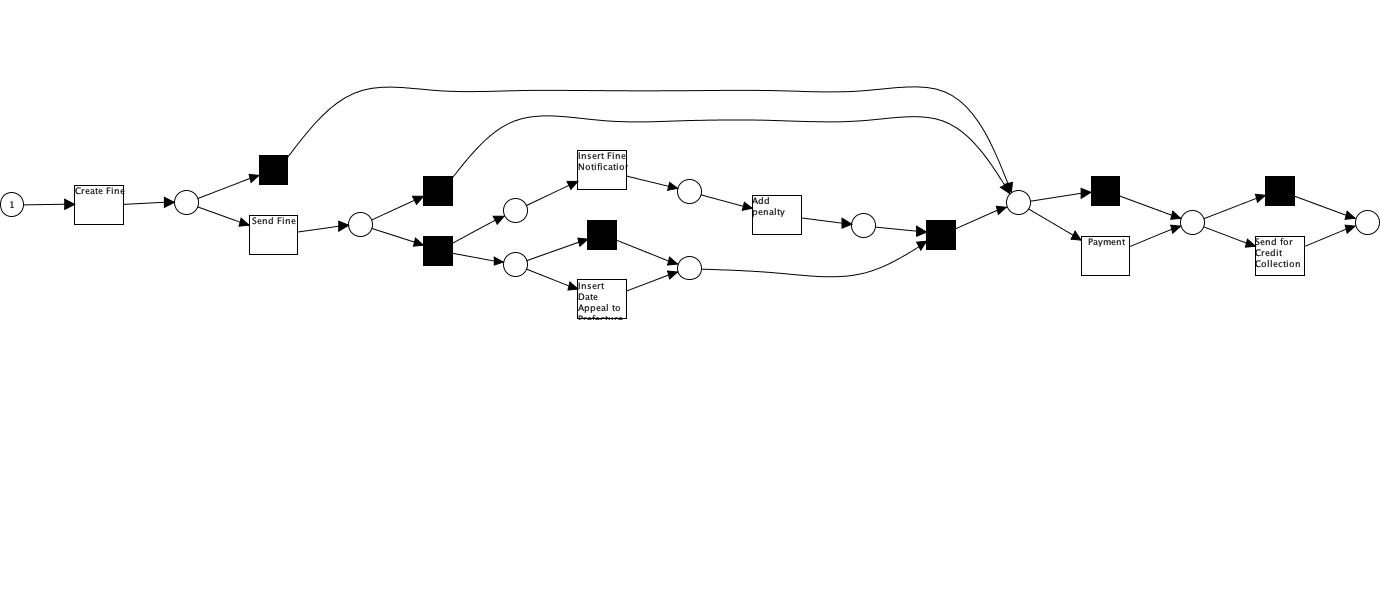
\includegraphics[width=\textwidth]{figures/im_no_appeals.png}
  \caption{Process model discovered from the log without any appeals using the inductive miner.}
  \label{fig:im_no_appeals}
\end{figure}

\paragraph{\textbf{b)}}

\paragraph{\textbf{c)}}

\paragraph{\textbf{d)}}

\paragraph{\textbf{e)}}

\section{Q3. Attribute Analysis and Compliance}

\section{Q4. Performance}

\section{Q5. Summary and Conclusion}

\section*{Appendix}

\begin{table}[H]
\centering
\begin{tabular}{|l|l|l|l|l|}
\hline \textbf{Activity} & \textbf{Complete} & \textbf{Only Appeals} & \textbf{Without Appeals} \\
\hline Add penalty & 79860 & 4357 & 75503\\
\hline Appeal to Judge & 555 & 555 &0\\
\hline Create Fine & 150370 & 4513 & 145857\\
\hline Insert Date Appeal to Prefecture & 4188 & 4146 & 42\\
\hline Insert Fine Notification & 79860 & 4357 & 75503\\
\hline Notify Result Appeal to Offender & 896 & 863 & 33\\
\hline Payment  & 77601 & 903 & 76698\\
\hline Receive Result Appeal from Prefecture & 999 & 964 & 35\\
\hline Send Appeal to Prefecture  & 4141 & 4141 & 0\\
\hline Send Fine  & 103987 & 4513 & 99474\\
\hline Send for Credit Collection & 59013 & 412 & 58601\\
\hline
\end{tabular}
\caption{Absolute Frequencies of Activities in the Event Logs}
\label{tab:1c_absolut}
\end{table}

\begin{table}[H]
\centering
\begin{tabular}{|l|l|l|l|l|}
\hline \textbf{Activity} & \textbf{Complete} & \textbf{Only Appeals} & \textbf{Without Appeals} \\
\hline Add penalty & 0.142234 & 0.146582 & 0.141991\\
\hline Appeal to Judge & 0.000988 & 0.018672 &0\\
\hline Create Fine & 0.267815 & 0.151830 & 0.274298\\
\hline Insert Date Appeal to Prefecture & 0.007459 & 0.139483 & 0.000079\\
\hline Insert Fine Notification & 0.142234 & 0.146582 & 0.141991\\
\hline Notify Result Appeal to Offender & 0.001596 & 0.029034 & 0.000062\\
\hline Payment  & 0.138210 & 0.030379 & 0.144238\\
\hline Receive Result Appeal from Prefecture & 0.001779 & 0.032432 & 0.000066\\
\hline Send Appeal to Prefecture  & 0.007375 & 0.139315 & 0\\
\hline Send Fine  & 0.185205 & 0.151830 & 0.187071\\
\hline Send for Credit Collection & 0.105104 & 0.013861 & 0.110205\\
\hline
\end{tabular}
\caption{Relative Frequencies of Activities in the Event Logs}
\label{tab:1c_relative}
\end{table}

\begin{table}[H]
\centering
\begin{tabular}{|l|l|l|l|l|}
\hline \textbf{Activity} & \textbf{Complete} & \textbf{Only Appeals} & \textbf{Without Appeals} \\
\hline Payment  & 0.446904 & 0.154443 & 0.455953\\
\hline Send for Credit Collection & 0.392346 & 0.087747 & 0.401770\\
\hline Send Fine  & 0.138026 & 0.001551 & 0.142249\\
\hline Send Appeal to Prefecture  & 0.020908 & 0.696654 & 0\\
\hline Appeal to Judge & 0.000891 & 0.029692 &0\\
\hline Notify Result Appeal to Offender & 0.000572 & 0.018170 & 0.000027\\
\hline Receive Result Appeal from Prefecture & 0.000352 & 0.011744 & 0\\
\hline
\end{tabular}
\caption{Fraction of Traces that end with the Corresponding Activity}
\label{tab:1c_end}
\end{table}

\end{document}

